\section{Fundamentação teórica}
\label{sec:fundamentacao}

O desenvolvimento de veículos inteligentes envolve a integração de diferentes conceitos relacionados à percepção do ambiente, à localização, ao planejamento de movimento e ao controle, sendo necessária uma arquitetura unificada e eficiente para executar todas as tarefas. Nesta seção, são apresentados os fundamentos teóricos necessários à compreensão da solução desenvolvida, abrangendo o modelo cinemático de bicicleta, o posicionamento GNSS (Sistema Global de Navegação por Satélite) com correções RTK (Cinemática em Tempo Real), a estimação de estados por filtro de Kalman estendido, o controle de trajetória pelo método Stanley \citep{Thrun2006}, além de exemplos de veículos autônomos e suas respectivas arquiteturas de sistema.

\subsection{Modelo cinemático de bicicleta}
\label{subsec:modelo_bicicleta}

A modelagem matemática do movimento de veículos terrestres permite descrever seu comportamento a partir das relações entre posição, orientação, velocidade e esterçamento. Entre as representações utilizadas para essa finalidade, destaca-se o modelo cinemático de bicicleta, que simplifica a geometria de direção Ackermann de um veículo de quatro rodas por meio de duas rodas equivalentes, posicionadas nos centros dos eixos dianteiro e traseiro \citep{Snider2009}. 

O modelo considera o movimento do veículo em um plano bidimensional, assumindo a condição derolamento sem deslizamento lateral dos pneus. Dessa forma, os efeitos dinâmicos associados às forças laterais, à transferência de carga e à interação entre os pneus e o solo, não são representados explicitamente. Essa aproximação é especialmente adequada para descrever o movimento de veículos em condições de baixa velocidade e manobras nas quais os efeitos de deslizamento lateral podem ser desprezados. 

Considerando um veículo com tração traseira e adotando o centro do eixo traseiro como ponto de referência, seu movimento pode ser descrito por:

\begin{equation}
\label{eq:modelo_cinematico}
\left\{
\begin{aligned}
\dot{x} &= v\cos(\theta) \\
\dot{y} &= v\sin(\theta) \\
\dot{\theta} &= \frac{v}{L}\tan(\delta)\\
\end{aligned}
\right.
\end{equation}

em que $x$ e $y$ representam as coordenadas da posição do veículo no referencial global, $\theta$ corresponde ao ângulo de orientação em relação a esse referencial, $v$ é a velocidade linear, $L$ representa a distância entre os eixos dianteiro e traseiro e $\delta$ corresponde ao ângulo de esterçamento equivalente das rodas dianteiras.

\begin{figure}[htb]
    \centering
    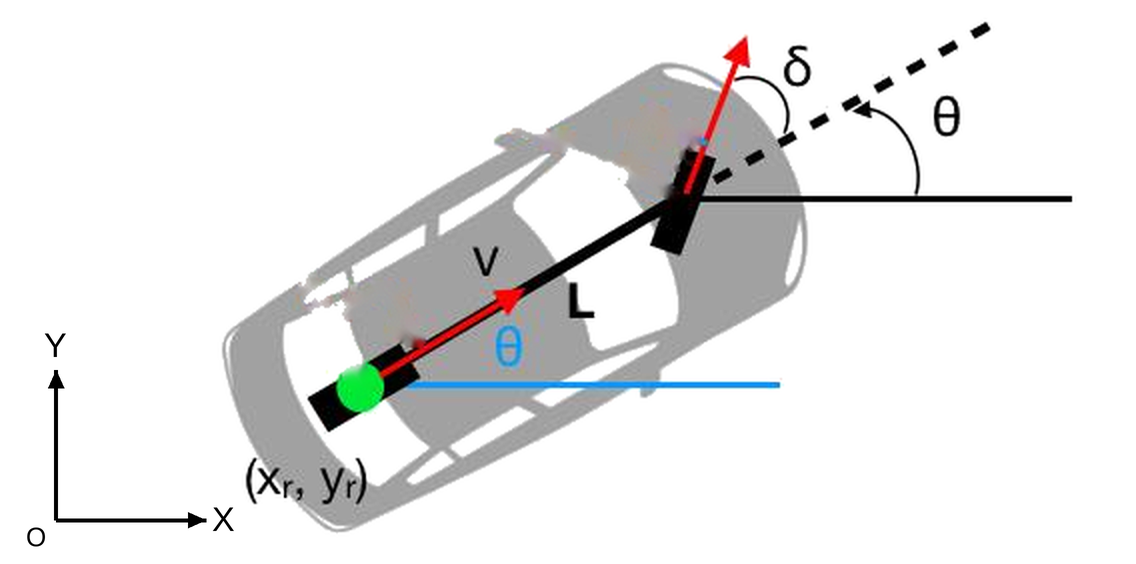
\includegraphics[width=0.85\columnwidth]{Imagens/Modelo cinemático de bicicleta.png}
    \caption{Representação geométrica do modelo cinemático de bicicleta. Fonte: \citet{Snider2009}.}
    \label{fig:modelo_bicicleta}
\end{figure}

As equações descrevem as velocidades de translação e de rotação do veículo em função da velocidade longitudinal e do ângulo de esterçamento. A partir da integração dessas relações ao longo do tempo, é possível determinar a evolução da posição e da orientação do veículo. Em particular, a taxa de variação da orientação depende diretamente da velocidade e da tangente do ângulo de esterçamento, sendo inversamente proporcional à distância entre os eixos \citep{Snider2009,Massera2014}. 

Embora simplificado, o modelo cinemático de bicicleta fornece uma representação matemática útil para o estudo da movimentação de veículos terrestres, constituindo uma base para o desenvolvimento de estratégias de localização, estimação de estados e controle de trajetórias.

\subsection{Posicionamento GNSS com RTK}

Os sistemas globais de navegação por satélite (\textit{Global Navigation Satellite Systems} -- GNSS) permitem determinar a posição de um receptor a partir de sinais transmitidos por diferentes constelações de satélites, como o GPS, dos Estados Unidos, o GLONASS, da Rússia, o Galileo, da União Europeia, e o BeiDou, da China. Entretanto, a precisão do posicionamento convencional é limitada por fatores como eerros orbitais e erros nos relógios dos satélites e dos receptores, atrasos atmosféricos e efeitos de multicaminhamento dos sinais. 
 
Para aplicações que exigem maior precisão, destaca-se a técnica RTK (\textit{Real-Time Kinematic}), baseada no posicionamento relativo entre um receptor móvel (\textit{rover}) e uma estação de referência com coordenadas conhecidas. A técnica utiliza observações da fase da portadora dos sinais GNSS e informações de correção para reduzir erros comuns às medições, possibilitando precisão centimétrica em condições favoráveis \citep{Bisnath2020}.  

A transmissão dessas correções pode ser realizada por meio do protocolo NTRIP (\textit{Networked Transport of RTCM via Internet Protocol}), que permite distribuir dados GNSS em tempo real pela internet. Nesse processo, as informações disponibilizadas por estações de referência são encaminhadas ao receptor móvel, permitindo a aplicação das correções durante o posicionamento \citep{BKG2026NTRIP}. 
 
A qualidade da solução RTK depende de fatores como a disponibilidade de sinais GNSS, a qualidade das observações e o recebimento adequado das correções. Entre os estados possíveis estão o RTK \textit{float}, no qual as ambiguidades da fase da portadora ainda não foram resolvidas como valores inteiros, e o RTK \textit{fixed}, no qual essa resolução foi obtida, permitindo maior precisão de posicionamento \citep{Ublox2025ZEDF9R}.

\subsection{Filtro de Kalman Estendido}
\label{subsec:fund_ekf}

A estimação de estados desempenha um papel fundamental em sistemas de navegação autônoma, uma vez que as medições dos sensores estão sujeitas a ruídos e incertezas. O filtro de Kalman é um estimador recursivo que combina informações de um modelo matemático com observações do sistema, considerando as incertezas associadas a ambas as fontes \citep{Welch2006}. 

O filtro de Kalman estendido (\textit{Extended Kalman Filter} -- EKF) permite aplicar essa abordagem a sistemas não lineares, por meio da linearização local dos modelos de movimento e observação por meio de matrizes jacobianas. Seu funcionamento é dividido em duas etapas principais: predição e correção \citep{Welch2006,Thrun2006}. 

Na etapa de predição, o estado estimado é propagado a partir do modelo de movimento: 

\begin{equation}
    \hat{\mathbf{x}}_{k}^{-} =
    f(\hat{\mathbf{x}}_{k-1},\mathbf{u}_{k-1}),
    \label{eq:ekf_predicao}
\end{equation}

em que $\hat{\mathbf{x}}_{k}^{-}$ representa a estimativa do estado antes da incorporação de uma nova medição, $f$ corresponde ao modelo não linear de movimento e $\mathbf{u}_{k-1}$ representa as entradas do sistema. 

A covariância associada à predição é calculada por:

\begin{equation}
    \mathbf{P}_{k}^{-} =
    \mathbf{F}_{k}\mathbf{P}_{k-1}
    \mathbf{F}_{k}^{T}+\mathbf{Q}_{k},
    \label{eq:ekf_cov_predicao}
\end{equation}

em que $\mathbf{F}_{k}$ é a matriz jacobiana do modelo de movimento, $\mathbf{P}_{k-1}$ é a covariância da estimativa anterior e $\mathbf{Q}_{k}$ representa a covariância do ruído de processo. 

Na etapa de correção, as medições dos sensores são incorporadas à estimativa por meio do ganho de Kalman: 

\begin{equation}
    \mathbf{K}_{k} =
    \mathbf{P}_{k}^{-}\mathbf{H}_{k}^{T}
    \left(
    \mathbf{H}_{k}\mathbf{P}_{k}^{-}
    \mathbf{H}_{k}^{T}+\mathbf{R}_{k}
    \right)^{-1} \,.
    \label{eq:ekf_ganho}
\end{equation}

A estimativa do estado é então atualizada por:

\begin{equation}
    \hat{\mathbf{x}}_{k} =
    \hat{\mathbf{x}}_{k}^{-}+
    \mathbf{K}_{k}
    \left[
    \mathbf{z}_{k}-
    h(\hat{\mathbf{x}}_{k}^{-}) 
    \right],
    \label{eq:ekf_correcao}
\end{equation}

em que $\mathbf{H}_{k}$ é a matriz jacobiana do modelo de observação, $\mathbf{R}_{k}$ representa a covariância do ruído de medição, $\mathbf{z}_{k}$ corresponde às observações dos sensores e $h$ representa o modelo não linear de observação. 

Por fim, a matriz de covariância é atualizada pela forma de Joseph, que contribui para a preservação de suas propriedades matemáticas diante de erros numéricos: 

\begin{equation}
\begin{aligned}
    \mathbf{P}_{k} ={}&
    (\mathbf{I}-\mathbf{K}_{k}\mathbf{H}_{k})
    \mathbf{P}_{k}^{-}
    (\mathbf{I}-\mathbf{K}_{k}\mathbf{H}_{k})^{T}\\
    &+\mathbf{K}_{k}\mathbf{R}_{k}\mathbf{K}_{k}^{T}\,.
\end{aligned}
    \label{eq:ekf_cov_correcao}
\end{equation}

Sendo assim, o EKF permite combinar informações de diferentes sensores, ponderando suas contribuições de acordo com as incertezas associadas ao modelo de movimento e às medições. Em sistemas de navegação terrestre, essa abordagem possibilita estimar variáveis como posição, orientação e velocidade \citep{Thrun2006}. 

\subsection{Controlador Stanley}

O controlador Stanley é um método de controle lateral não linear utilizado para o seguimento de trajetórias em veículos autônomos. Desenvolvido pela equipe da Universidade de Stanford, o método foi empregado no veículo vencedor do DARPA Grand Challenge de 2005 \citep{Thrun2006}. 

Sua formulação considera dois erros geométricos: o erro de orientação ($\psi$), definido pela diferença angular entre a direção da trajetória de referência e a orientação do veículo, e o erro lateral ($e$), correspondente ao deslocamento transversal do centro do eixo dianteiro em relação à trajetória desejada \citep{Thrun2006}. 

\begin{figure}[htb]
    \centering
    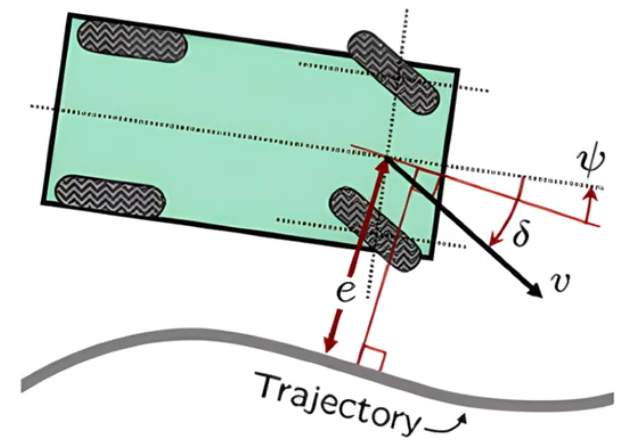
\includegraphics[width=0.85\columnwidth]{Imagens/Controlador Stanley.png}
    \caption{Representação geométrica do controlador Stanley. Fonte: \citet{Hoffmann2007}.}
    \label{fig:controlador_stanley}
\end{figure}

Adotando-se a convenção de que o erro lateral é positivo quando o veículo se encontra à esquerda da trajetória de referência, a lei de controle pode ser expressa por:

\begin{equation}
    \delta =
    \psi -
    \arctan\left(\frac{k e}{v}\right),
    \label{eq:stanley}
\end{equation}

em que $\delta$ representa o ângulo de esterçamento comandado, $k$ é um ganho positivo de controle e $v$ corresponde à velocidade longitudinal do veículo. 

O primeiro termo atua no alinhamento da orientação do veículo com a trajetória, enquanto o segundo corrige o deslocamento lateral. A influência desse último termo diminui com o aumento da velocidade, para um mesmo erro lateral \citep{Hoffmann2007}. 

Em aplicações práticas, a formulação pode incorporar modificações destinadas a melhorar o comportamento do controlador. Entre elas, destaca-se a introdução de um parâmetro de suavização $k_s$ no denominador, que limita a sensibilidade da correção lateral em velocidades próximas de zero \citep{Hoffmann2007}. 

Além disso, pode-se empregar uma ação antecipativa (\textit{feedforward}) baseada na curvatura $\kappa$ da trajetória, utilizando a relação geométrica entre a curvatura e o esterçamento. Essa compensação pode ser expressa por: 

\begin{equation}
    \delta_{ff} =
    k_{ff}\arctan(L_{ff}\kappa),
    \label{eq:stanley_feedforward}
\end{equation}

em que $k_{ff}$ representa o ganho antecipativo e $L_{ff}$ corresponde à distância entre eixos considerada na compensação da curvatura. Também podem ser incorporados termos de amortecimento relacionados à velocidade angular do veículo, com o objetivo de reduzir oscilações do comando de esterçamento \citep{Hoffmann2007}. 

Dessa forma, o método Stanley permite determinar o esterçamento a partir dos desvios geométricos em relação à trajetória, podendo ser complementado por estratégias que considerem a curvatura do percurso e o comportamento da orientação do veículo. 

\subsection{Exemplos de Arquiteturas de Veículos Autônomos}
\label{subsec:arquiteturas_referencia}

O desenvolvimento de veículos autônomos exige a integração de diferentes subsistemas responsáveis por percepção, localização, planejamento e controle. Para organizar essas funções, diferentes plataformas experimentais adotam arquiteturas modulares e distribuídas, permitindo separar responsabilidades, estabelecer mecanismos de comunicação e integrar componentes com diferentes requisitos computacionais.

O veículo Stanley, desenvolvido pela Universidade de Stanford, utilizava uma arquitetura distribuída, organizada em módulos de software responsáveis por funções como percepção do ambiente, localização, planejamento e controle. Essa organização permitia executar diferentes processos de maneira integrada, combinando informações dos sensores com as decisões de navegação e os comandos de atuação do veículo \citep{Thrun2006}.

No Brasil, o projeto CaRINA, desenvolvido pela Universidade de São Paulo (USP), adotou uma arquitetura modular baseada no ROS, permitindo integrar componentes de hardware e software por meio de mecanismos padronizados de comunicação. Essa abordagem favoreceu o desenvolvimento independente dos subsistemas e sua integração em diferentes configurações experimentais \citep{Fernandes2014}.

O veículo IARA, desenvolvido pela Universidade Federal do Espírito Santo (UFES), também apresenta uma arquitetura organizada em subsistemas especializados, abrangendo percepção, localização, tomada de decisão, planejamento de movimento e controle. A integração desses componentes permite transformar as informações obtidas pelos sensores em decisões de navegação e comandos de atuação, possibilitando a operação autônoma do veículo \citep{Badue2021}.